%==============================================================================
%  The geography of residential access after a permanent mid-grid cut
%  Original research article for Journal of Transport Geography (Elsevier).
%
%  Class:  cas-dc [a4paper,fleqn]
%            Elsevier CAS double-column
%            natbib author-year (cas-model2-names)
%
%  Build:  .\build.ps1
%==============================================================================

\documentclass[a4paper,fleqn]{cas-dc}

\usepackage[authoryear,longnamesfirst]{natbib}
\usepackage{graphicx}
\usepackage{booktabs}
\usepackage{tabularx}
\usepackage{array}
\usepackage{amsmath}
\usepackage{amssymb}
\usepackage{flafter}
\usepackage{ragged2e}

\graphicspath{{../figures/}}

\newcolumntype{Y}[1]{>{\RaggedRight\arraybackslash}p{#1}}
\renewcommand{\arraystretch}{1.08}
\setlength{\tabcolsep}{4pt}

\begin{document}
\let\WriteBookmarks\relax
\setcounter{topnumber}{3}
\setcounter{dbltopnumber}{2}
\setcounter{bottomnumber}{1}
\setcounter{totalnumber}{4}
\renewcommand{\topfraction}{0.92}
\renewcommand{\dbltopfraction}{0.95}
\renewcommand{\bottomfraction}{0.45}
\renewcommand{\textfraction}{0.05}
\renewcommand{\floatpagefraction}{0.85}
\renewcommand{\dblfloatpagefraction}{0.85}
\setlength{\floatsep}{8pt}
\setlength{\textfloatsep}{10pt}
\setlength{\intextsep}{8pt}
\setlength{\dblfloatsep}{8pt}
\setlength{\dbltextfloatsep}{10pt}
\raggedbottom
\makeatletter
\setlength{\@fptop}{6pt}
\setlength{\@fpsep}{10pt}
\setlength{\@fpbot}{0pt plus 1fil}
\setlength{\@dblfptop}{6pt}
\setlength{\@dblfpsep}{10pt}
\setlength{\@dblfpbot}{0pt plus 1fil}
\makeatother

\shorttitle{Residential access after a mid-grid cut}
\shortauthors{Moode}

\title[mode=title]{The geography of residential access after a permanent
mid-grid cut: Barcelona's Eixos Verds}

\author[1]{Seshadri Naik Moode}
\cormark[1]
\ead{seshadri.naik.moode@upc.edu}
\ead[url]{https://orcid.org/0000-0002-9651-7535}
\credit{Conceptualization, Methodology, Software, Formal analysis,
Validation, Visualization, Writing -- original draft,
Writing -- review \& editing}
\affiliation[1]{organization={Barcelona Innovative Transportation (BIT),
Universitat Polit\`ecnica de Catalunya -- BarcelonaTech (UPC)},
            addressline={Jordi Girona 1--3},
            city={Barcelona},
            postcode={08034},
            country={Spain}}
\cortext[1]{Corresponding author. ORCID: 0000-0002-9651-7535}

\begin{abstract}
Closing a street to through traffic is not the same as sacrificing access
to other residents. This article estimates the change in intra-municipal
residential interaction potential after a counterfactual through-movement
recode of Barcelona's first permanent Eixos Verds: 4.85\,km of as-built
green axes on the Cerd\`a grid. Travel times are simulated free-flow
shortest paths on one OpenStreetMap extract. Accessibility is cumulative
opportunity to 2022 census-section population, checked with Hansen gravity.
Jobs, shops and a mixed-use 15-minute-city amenity layer are a different
destination mass and are not estimated. Two post-car graphs bound the recode
(treated-edge time $\times 100$, and treated edges removed). A third adds a
stated 15\,s penalty on non-through turns, pre and post. Centroids that land
on a treated node are connected to the nearest untreated perpendicular.

For 1{,}052 off-axis origins the median 15-minute car loss is $0$ under
$\times 100$ and $-0.10\%$ when treated edges are dropped. A 15\,s turn
penalty leaves that 15-minute median at $0$. Nobody gains. Hansen moves by
$-0.018\%$. On this grid the recode barely moves residential interaction
potential inside the municipality. The geographical object is incidence of
that small change.
\end{abstract}

\begin{highlights}
\item Off-axis 15-min residential car: $0$ ($\times 100$) or $-0.10\%$ (drop).
\item A stated 15\,s turn penalty leaves the 15-min median at $0$.
\item Hansen off-axis median is $-0.018\%$; nearby still ranks first.
\item Local egress snaps replace centroids trapped on the treated centreline.
\item Drop-treated is $-0.10\%$ in every district.
\end{highlights}

\begin{keywords}
residential accessibility \sep cumulative opportunity \sep Hansen \sep
road-space reallocation \sep Eixos Verds \sep Barcelona \sep
interaction potential \sep through-movement
\end{keywords}

\maketitle
\raggedbottom

%==============================================================================
\section{Introduction}
%==============================================================================

When a city removes through-movement from a street, two questions arrive
together and are then confused. Did traffic fall? And did people lose access
to the rest of the city? Point counts can speak to the first. They cannot
speak to the second. A loop records vehicles, not opportunities reached. A
short extra detour on a redundant grid can leave 15-minute catchments almost
intact while still rearranging who sits on the last minute of an isochrone.
Treating a local volume drop as an accessibility result is a category error
--- the gap this article fills. Counts, emissions and safety remain
policy objects; they are complementary, not dismissed, and they are not
estimated here.

Accessibility is the ease of reaching valued destinations
\citep{Hansen1959,Geurs2004,Paez2012,Wu2020}. It is a geographical quantity:
it lives at origins, decays with travel time or cost, and is uneven across
the city \citep{Kwan1998,Miller1999,Neutens2015}. That geography is the
reason a city-mean delay is the wrong summary. The people who lose a
destination at 14 minutes 50 seconds are not the same people who live on the
closed street, and they are not a random sample of the municipality.
Road-space reallocation, low-traffic neighbourhoods and superblocks are
usually evaluated on counts, speeds, or health
\citep{Cairns1998,Cairns2002,NelloDeakin2022,Thomas2024,Mueller2020,Banister2008}.
The 15-minute-city vocabulary \citep{Moreno2021,Pozoukidou2021} has made
access politically salient, and has made 15 minutes the cutoff cities
recognise. That cutoff is used here as a time threshold on residential
interaction potential, not as a mixed-use amenity claim and not as a test of
whether Barcelona is a 15-minute city. Destinations are 2022 residents:
Hansen's interaction potential \citep{Hansen1959}, not shops or jobs. An
amenity or workplace layer is a different destination mass and a different
paper. This article asks whether a permanent mid-grid through-cut changes
\emph{car} opportunity to other residents, and who bears that change.

Barcelona's first Eixos Verds (green axes) are a clean test on the Cerd\`a
grid (Fig.~\ref{fig:study}).
In 2022--23 the city converted a tactical layout into a permanent forced-turn
geometry: Consell de Cent from Vilamar\'i to Passeig de Sant Joan, short
stretches of Girona, Rocafort and Comte Borrell, and four squares at the
crossings --- 4.85\,km of as-built principal centreline, all inside the
Eixample. Through-movement on those axes was designed out.
\citet{NelloDeakin2022} already showed that tactical versions of nearby
streets could cut local average daily traffic. That local-volume result is
taken as given and is not re-estimated. This article asks a different
question, on a counterfactual recode of the permanent geometry: how does
opportunity accessibility change, and who bears the change?

The contribution is a labelled accessibility account on a citywide
network-distance graph, not a prettier isochrone and not a city-mean delay.
A 15-minute catchment drawn once, for one origin, can illustrate the
mechanism (Fig.~\ref{fig:isochrones}); it cannot be the result.
\begin{enumerate}
\item Simulated origin--destination travel time, car and walk, on a municipal
OpenStreetMap extract rather than a corridor clip;
\item Estimated cumulative-opportunity accessibility at every census section,
with Hansen gravity at $\beta = 0.05$ per minute as an uncalibrated ranking
check;
\item Incidence of that change by network distance, neighbourhood and
household income;
\item A stated 15\,s time penalty on non-through turns, applied to both pre
and post car graphs. It is topological friction, not a signalised cycle and
not a probe-speed assignment.
\end{enumerate}
Pre and post are two recodes of \emph{one} contemporary graph. They are not
two dated OpenStreetMap extracts. The dependent time is uncongested
shortest-path time on that graph: the object is the geography of a
through-cut on a redundant grid, not peak-hour congested accessibility.
Traffic counts, vehicle-kilometres and evaporative demand are outside the
objects. Opportunities are 2022 resident population. Household disposable
income per capita (2022) is joined only for incidence. Walk access is
reported as a level on an unchanged pedestrian graph. Walk \emph{change} is
zero by construction until a green-axis speed-up is written as a stated
scenario; that scenario is not run here.

Section~\ref{sec:lit} places accessibility after a cut against the volume
literature, the measurement of opportunity, and the 15-minute-city claim.
Section~\ref{sec:case} describes phase~1 and the data.
Section~\ref{sec:method} defines the graphs, the through-movement proxies,
and $A_i(t)$. Section~\ref{sec:results} reports corridor times, two worked
catchments, off-axis accessibility, neighbourhood and income incidence, and
the on-axis caveat. Section~\ref{sec:disc} states what can be claimed.
Section~\ref{sec:conc} concludes.

%==============================================================================
\section{Access, not volume, after a street is closed}
\label{sec:lit}

\subsection{Volume is not an accessibility result}

Taking road space from general traffic is an old sustainable-mobility
instrument \citep{Banister2008,Bertolini2005}. The evaluation that follows
is almost always a set of point counts. Local motor traffic often falls;
one-for-one displacement onto the nearest parallel is not a general law;
travellers adapt on route, time, mode and destination
\citep{Cairns1998,Cairns2002,NelloDeakin2022,Thomas2024,Tennoy2021,Parady2025}.
Network vehicle-kilometres after \emph{permanent} cuts remain thinly measured
in an agency evidence review \citep{Koorey2025}. Boundary-road congestion is
a related but distinct
object \citep{Verlinghieri2025}. None of that is an accessibility result. A
count residual called evaporation does not say whether the remaining trips
still reach the same opportunities in the same time. A city can record fewer
vehicles on the treated street and still have left 15-minute catchments
almost intact, or the reverse. Those two sentences can both be true; they
are not substitutes. Volume, congestion, emissions and safety remain
relevant for a street-closure decision; they are a different matrix, and
they are not estimated in this article.

\subsection{Opportunity, cutoffs, and gravity}

\citet{Hansen1959} defined accessibility as potential for interaction,
discounted by impedance. Reviews since then have insisted on the same
components --- land use, the transport system, a temporal constraint, and an
individual or zonal unit --- and on the ease with which the word is used for
something else \citep{Geurs2004,Paez2012,Handy2020,Wu2020}. Cumulative
opportunity, the mass of destinations inside a time threshold, is the
indicator cities now recognise as a ``15-minute'' catchment
\citep{Moreno2021}. It is geographically sharp and statistically brittle: a
destination that sits at 14 minutes 50 seconds is in; at 15 minutes 10
seconds it is out. Gravity or Hansen forms avoid the knife-edge by giving
every destination a positive but decaying weight
\citep{Geurs2004,Paez2012}. Space--time measures make the same point at the
person rather than the zone \citep{Kwan1998,Miller1999}. This article uses
cumulative opportunity as the primary map because 15 minutes is the
threshold cities now print, and Hansen as the check that must reverse any
ranking produced only by the cutoff. If the two maps tell different geographical
stories, the cutoff --- not the detour --- is doing the work. That is a
geographical claim about an indicator, not a mixed-use 15-minute-city
evaluation.

Plans invoke accessibility more often than they operationalise it
\citep{Boisjoly2017}. Walking and cycling accessibility have their own
operational literature \citep{Vale2016,Marquet2015}. They do not replace a
pre/post car-opportunity account on the same network after a through-movement
cut. Superblock evaluations that report walkability or health gains
\citep{Mueller2020} answer a different question, on a different object.

\subsection{Equity as incidence}

Equity here means incidence of $\Delta A$: who sits where the change is
larger \citep{Pereira2017,Neutens2015,Lucas2012,Martens2017,Foth2013}. It is
not a second welfare theory and it is not a Gini of accessibility levels.
If a 15-minute map darkens the urban edge while a Hansen map darkens the
blocks next to the cut, the geography of the \emph{indicator} has been
mistaken for the geography of the \emph{detour}. Income can still be joined,
but only to test whether that ranking is a poverty penalty or a coincidence
of where poorer census sections sit on this grid. A correlation of
$\%\Delta A$ with network distance is topological: it says whether the map
is a cutoff or a detour. It is not a causal claim about economic or social
impacts after controlling for unobserved spatial heterogeneity.
\citet{Handy2020} warned
that accessibility is easy to invoke and easy to mis-measure. The mis-measure
in this setting is a choropleth of a round threshold, read as an equity
result.

The 15-minute city is a proximity claim about daily destinations
\citep{Moreno2021,Pozoukidou2021}. This article uses the 15-minute
\emph{cutoff}, because that is the threshold cities now print, not because
shops and jobs are in the destination mass, and not as an evaluation of
15-minute-city viability. Barcelona already has a dense,
mixed Eixample in which many daily destinations lie inside a short walk
\citep{Marquet2015}. That fact makes the car-opportunity question sharper,
not weaker: if the grid is redundant, a mid-block through-cut should barely
move car catchments to other residents; if it is not, the 15-minute map
should darken next to the axes. Those are empirical alternatives. They
cannot be read off a volume count. They also do not generalise, without
further work, to a dendritic suburb or a single-carriageway high street
\citep{Thomas2024,Parady2025,Verlinghieri2025}. The boundary condition is
the Cerd\`a grid.

Table~\ref{tab:objects} states the objects. Opportunities are residents:
Hansen's original interaction potential. Census sections are both origins
and destinations, with $T_{ii}=0$; own-zone population is included and is a
non-trivial share of walk $A_i$. A workplace or amenity layer would change
\emph{levels} of $A_i$ and might change incidence. Transit timetables and a
walk speed-up on the green axes are excluded for the same reason: they are
not in the recode. Probe speeds and a user-equilibrium assignment are
excluded for the same reason: they would identify a different time, not a
tighter version of this recode.

\begin{table*}[t]
\centering
\small
\caption{What this article measures, and what it does not.}
\label{tab:objects}
\begin{tabular}{Y{3.0cm}Y{4.0cm}Y{3.0cm}Y{4.0cm}}
\toprule
Object & Status & Object & Status \\
\midrule
Shortest-path time $T_{ij}$
  & Simulated, free-flow recode
  & Traffic counts / VKT
  & Complementary; not estimated \\
Cumulative opportunity $A_i(t)$
  & Estimated from simulated times
  & Jobs, shops, GTFS
  & Different destination mass \\
Hansen $H_i$ ($\beta = 0.05$ / min)
  & Uncalibrated ranking check; $0.03$ and $0.15$ as stated bounds
  & Congested assignment / probes
  & Different time object \\
20\% slower Consell-aligned parallels
  & Stated free-flow sensitivity
  & Household income (2022 RDLpc)
  & Off-axis quintiles only \\
15\,s non-through turns, pre and post
  & Stated turn-cost recode
  & Walk graph
  & Unchanged; walk $A_i$ is a level \\
Local egress to untreated perpendiculars
  & 15 treated-node centroids
  & Adjacent-municipality population
  & Not in $O_j$ \\
\bottomrule
\end{tabular}
\end{table*}

%==============================================================================
\section{Case and data}
\label{sec:case}

Phase~1 of the Eixos Verds is the treatment (Fig.~\ref{fig:study}: ten
districts in (a); coral, the as-built 4.85\,km centreline, named in (b)). Works ran
from 16 August 2022 into spring 2023. The as-built principal centrelines used
here, and not rewritten, are Consell de Cent ($\sim$3.00\,km), Girona
(0.75\,km), Rocafort (0.60\,km) and Comte Borrell (0.50\,km):
4.85\,km undirected. The same streets had carried a tactical regime
from 2020. This article studies the permanent through-movement cut, not
Nello-Deakin's eleven COVID tactical streets, and does not re-estimate his
Euclidean-buffer design. The axes sit in three Eixample neighbourhoods
(Dreta, Nova Esquerra, Antiga Esquerra). Far districts --- Nou Barris, Sant
Andreu, the hills of Horta-Guinard\'o --- are in the study because they are
where a 15-minute car catchment already ends. Restricting origins to a
sausage around Consell de Cent would hide the cutoff artefact that the maps
are built to show.

\begin{figure*}[t]
\centering
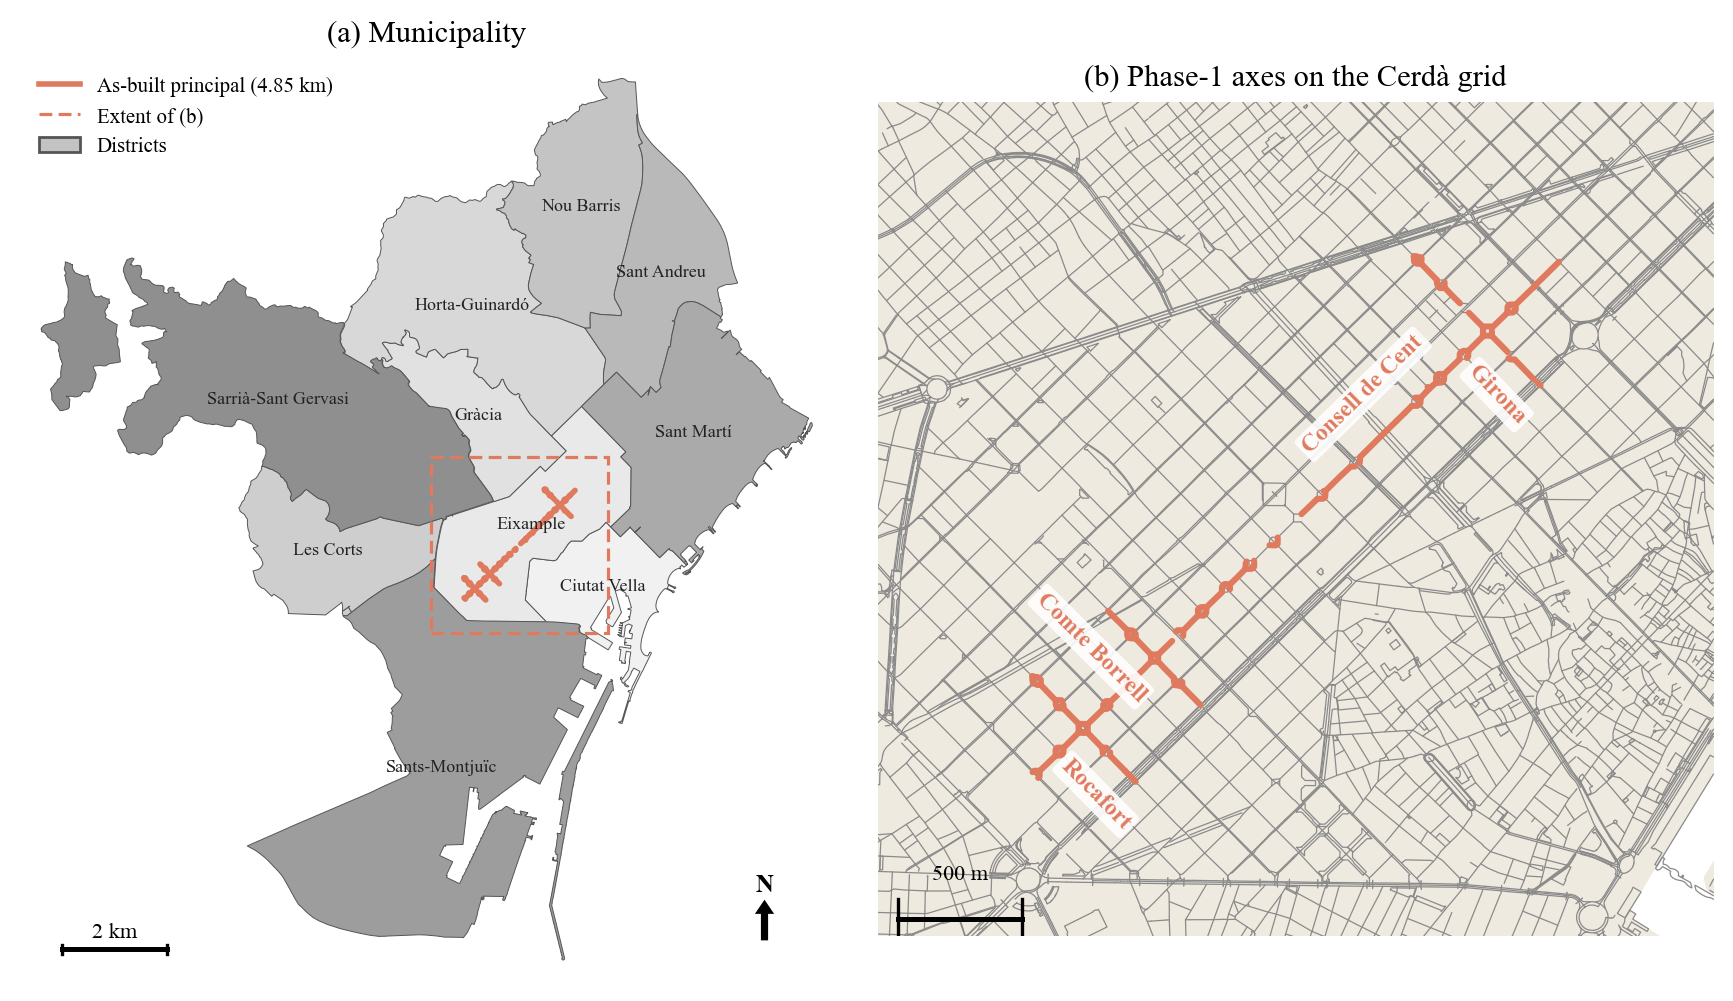
\includegraphics[width=\textwidth]{Fig1_study_area.png}
\caption{Barcelona (a) and as-built Eixos Verds phase~1 on the Cerd\`a grid
(b). Principal centreline 4.85\,km.}
\label{fig:study}
\end{figure*}

Origins and destinations are Barcelona's 1{,}068 census sections.
Opportunities $O_j$ are 1 January 2022 municipal \emph{padr\'o} population
(1{,}639{,}981 residents): residential interaction potential inside the
city, not the metropolitan first crown. A 15-minute car trip from Nou Barris
or Sants can reach Santa Coloma, Badalona or L'Hospitalet; those residents
are not in $O_j$. Levels of $A_i$ at the rim are therefore intra-municipal.
Neighbourhood (\emph{barri}) and district names
are used only to aggregate incidence. One car origin, section 7097 (Montbau,
869 residents), lies 331\,m from the nearest motorised node, in Collserola.
A centroid connector of that length would invent a driveway. The section is
left unsnapped on the car graph and remains on the walk graph.
Fifteen centroids land on a treated node. Those origins and destinations are
connected to the nearest untreated perpendicular Cerd\`a street within
200\,m (median snap 73\,m). That is local egress, not a through-movement on
the green axis.

The street network is a single OpenStreetMap highway extract covering the
municipal bbox (127{,}766 ways, retrieved 7 September 2026), clipped to the
union of neighbourhood polygons plus 300\,m. The graph therefore stops near
the municipal edge; adjacent municipalities are not a second destination
layer. Pre and post are recodes of
that graph, not two historical dumps. Current OSM has already retagged parts
of Consell de Cent off the motorised extract, so the as-built principal is
injected (9.84\,km directed injected; 12.03\,km directed treated).
A 3.5\,km clip around the axes would leave 241 sections, about 361{,}000
people, off the graph; 15 minutes at 20\,km/h is already about 5\,km. Car
edges follow motorway-through-living-street classes, with OSM
\texttt{maxspeed} where present and otherwise 80 / 50 / 40 / 30 / 20\,km/h
by hierarchy (injected principal 30\,km/h). Walk edges are pedestrian-usable
ways at 4.5\,km/h (steps 2\,km/h). Dijkstra weight is travel time,
not length. Times are uncongested; they are not matched to floating-car or
probe speeds. The object is relative $\Delta A$ under that free-flow graph,
not clock-time travel in peak Eixample. A corridor check below asks only
whether implied speed sits inside those defaults. A uniform junction delay
on every node would shift the \emph{level} of $T_{ij}$ and could pull
central 15-minute catchments off their municipal ceiling; it would not, by
itself, identify the through-cut unless that delay sat only on the recoded
geometry. The stated 15\,s and 30\,s dual already puts extra time on every
non-through turn, pre and post.

Census-section centroids snap to the giant weakly connected component (car
median snap 30.8\,m, $n = 1{,}067$; walk 17.5\,m, $n = 1{,}068$). Exposure
for incidence is undirected network distance on the pre-car graph to a
treated node. Euclidean distance is diagnostic only. Household disposable
income per capita for 2022 (Open Data BCN, RDLpc) joins on
$\mathrm{Codi\_Districte}\times 1000 + \mathrm{Seccio\_Censal}$ for all
1{,}068 sections; quintiles are computed on off-axis sections only.

%==============================================================================
\section{Method}
\label{sec:method}

\subsection{Through-movement recodes}

Let $G^{\mathrm{pre}}$ be the injected car graph. Treated edges are OSM
links whose midpoint is within 15\,m of the principal and whose heading
satisfies $|\cos\theta| \ge 0.8$, plus the injected centreline itself. The
15 on-axis origins are a property of that snap, not a land-use definition of
who lives on Consell de Cent. They are re-snapped to the nearest untreated
perpendicular before $A_i$ is estimated. Two post graphs bound the recode rather than
pretending that one penalty is the lived geometry.

\begin{itemize}
\item $\times 100$. Treated edges have time and length multiplied
by 100. This is an upper bound on car time loss for leaving a node
that sits on a treated edge. The finite penalty keeps the edge in the graph,
so Dijkstra can still leave a trapped node at a punitive cost. It is a
through-movement prohibition, not a calibrated delay.
\item Drop-treated. Treated edges are deleted --- the deactivated
edge that $\times 100$ only inflates. The giant weakly
connected component is retained; sections are re-snapped to
remaining nodes. Origins that sat only on treated nodes must not keep their
pre snap. After local egress, one section remains isolated on the drop graph
(Table~\ref{tab:stubborn}); that is a local-access caveat, not hidden.
\item Turns $+15$\,s. On both $G^{\mathrm{pre}}$ and the
$\times 100$ graph, a shortest path is computed on the directed-edge dual.
A non-through turn ($|\cos\theta| < 0.8$) adds 15\,s, a conservative delay
for an uncontested urban turning manoeuvre; a through movement adds none. The same rule applies pre and post. It is a stated topological
friction, not a signal delay and not a count of extra vehicles. The same
dual with a 30\,s non-through penalty is a stated bound: it tests whether
the Cerd\`a grid's redundancy survives a harsher turn cost.
\item Parallels $\times 1.2$. On the $\times 100$ graph, untreated
edges aligned with Consell de Cent ($|\cos\theta|\ge 0.8$) whose midpoint
lies 80--400\,m from the principal have time multiplied by 1.2 (1{,}533
directed edges, 32\,km). This is a stated free-flow delay on the Cerd\`a
parallels, not an assignment of extra vehicles.
\end{itemize}

Walk pre and post are the same graph (Table~\ref{tab:graphs}). A ``walk got
faster'' claim would require recoding treated edges as a stated pedestrian
scenario. That recode is not run. Cycle and transit wait on a cycle extract
and a GTFS layer; they are not mixed into the car table.

\begin{table}[!htbp]
\centering
\small
\caption{Directed graphs.}
\label{tab:graphs}
\setlength{\tabcolsep}{3pt}
\begin{tabular}{@{}lrr@{}}
\toprule
Graph & Nodes & Edges \\
\midrule
Car, pre (injected) & 79{,}893 & 109{,}238 \\
Car, post ($\times 100$) & 79{,}893 & 109{,}238 \\
Car, post (parallels $\times 1.2$) & 79{,}893 & 109{,}238 \\
Car, post (drop-treated) & 79{,}646 & 108{,}507 \\
Walk & 296{,}711 & 712{,}786 \\
\bottomrule
\end{tabular}
\end{table}

\subsection{Accessibility}

At origin $i$,
\begin{equation}
A_i(t) = \sum_j O_j \mathbf{1}[T_{ij} \le t],
\label{eq:cumopp}
\end{equation}
with $T_{ii} = 0$ (own-zone population is included). Thresholds: car 15 and
30 minutes; walk 15 minutes. The 15-minute car map is primary because that
is the political threshold; 30 minutes is the check that a thin isochrone
edge is not being sold as a network shock. From a central Eixample origin,
15 minutes of free-flow car time already reaches most of the municipal
population (section 2138: 1.59 million of 1.64 million). Cumulative
opportunity then sits near its municipal ceiling, so a small detour need not
move $A_i(15)$. That ceiling is a property of the indicator under free-flow
time on this graph, not a finding that the cut is invisible. Hansen has no
knife-edge. The Ciutat Meridiana catchment is already inside the 15-minute
rim, so it can lose a destination without sitting at the ceiling.
Hansen robustness, truncated at 30 minutes:
\begin{equation}
H_i = \sum_j O_j \exp(-\beta T_{ij}), \qquad
\beta = 0.05~\mathrm{min}^{-1}.
\label{eq:hansen}
\end{equation}
The decay is a ranking check on the same simulated times, not a
friction-of-distance fit to Barcelona trip lengths. The reported map uses
$\beta = 0.05$\,min$^{-1}$ (half-life about 14 minutes). Stated bounds
$\beta = 0.03$ and $\beta = 0.15$ ask whether nearby still ranks first when
the decay is flatter or steeper; they are not an EMEF calibration. Percentage change is
\begin{equation}
\%\Delta A_i = 100 \times
(A_i^{\mathrm{post}} - A_i^{\mathrm{pre}}) / A_i^{\mathrm{pre}}.
\label{eq:pct}
\end{equation}
Shortest paths are computed with Dijkstra on a compressed sparse time
matrix, origins and destinations being the snapped section nodes, cutoff
30 minutes. Link time is cruise time at OSM speeds. The primary $T_{ij}$
uses that link time. A stated dual-graph recode adds 15\,s at non-through
turns, pre and post (64{,}374 dual links carry the penalty). $T_{ij}$ is
simulated. $A_i$ is estimated. Neither is observed.

\subsection{Off-axis sample and incidence}

Off-axis origins are the 1{,}052 snapped sections that were never
on a treated node. Fifteen centroids that would have snapped onto a treated
node (23{,}479 residents) receive a local-egress connector and are mapped
separately (Fig.~\ref{fig:onaxis}). Headline numbers are off-axis medians. Incidence tables aggregate the same off-axis rows by
district, \emph{barri}, and 2022 RDLpc quintile. Correlation of $\%\Delta A$
with network distance is reported as a diagnostic of whether the map is a
cutoff or a detour. It is a complete-enumeration Pearson coefficient, not a
spatial-error model of incidence. Moran's $I$ under queen contiguity of the
off-axis sections is reported with a permutation $z$-score and pseudo
$p$-value (999 randomisations) with the same maps.

Two worked catchments (Fig.~\ref{fig:isochrones}) show the same mechanism at
the destination end. Destinations are census sections whose snap node lies
inside 15 minutes; they are not a continuous isochrone contour. One origin
sits 157\,m off the axes in Nova Esquerra de l'Eixample (section 2138). The
other sits in Ciutat Meridiana, Nou Barris (section 8111), at the far edge
of the municipal graph. If the 15-minute loss is a knife-edge, the second
origin should shed destinations in the centre of the city, not next to the
axes. If the loss is a local detour, the first origin should shed a handful
of nearby sections. Both can be true at once; they are different
geographies.

%==============================================================================
\section{Results}
\label{sec:results}
%==============================================================================

\subsection{Corridor time}

Opposite ends of the axis band (census sections 2136 and 2067, centroids
within 150\,m of the principal) give simulated car times of 4.1 minutes
pre and 4.8 minutes post under $\times 100$:
$+0.7$ minutes. With the 15\,s turn recode the same pair is 4.8
minutes pre and 5.9 minutes post ($+1.1$ minutes). Euclidean
separation is 2.8\,km. Those are recode-consistency checks on link time and
stated turn friction, not probe speeds. The Cerd\`a grid already supplies a
time-competitive parallel. The penalty binds; the detour is small.

\subsection{Two 15-minute catchments}

Fig.~\ref{fig:isochrones} draws the destination set of Eq.~\eqref{eq:cumopp}
for two origins, after local-egress snaps. From section 2138, 157\,m off the
axes in Nova Esquerra, 1{,}043 sections (1.59 million residents) lie inside
15 minutes before the cut. None of those sections leave the catchment after
$\times 100$. From section 8111 in Ciutat Meridiana the pre catchment is
already smaller (818 sections, 1.24 million people). One section, 2{,}076
people, leaves it --- inside Barcelona, at the far rim of a 15-minute car
trip from the northern edge. Adjacent municipalities sit outward of this
origin; the destination that leaves sits inward. Nobody is added to either
catchment. The near origin loses 0\% of reachable population; the far origin
loses $0.17\%$. Once destinations are not trapped on the treated centreline,
the 15-minute map no longer sheds a dozen central sections.

\begin{figure*}[t]
\centering
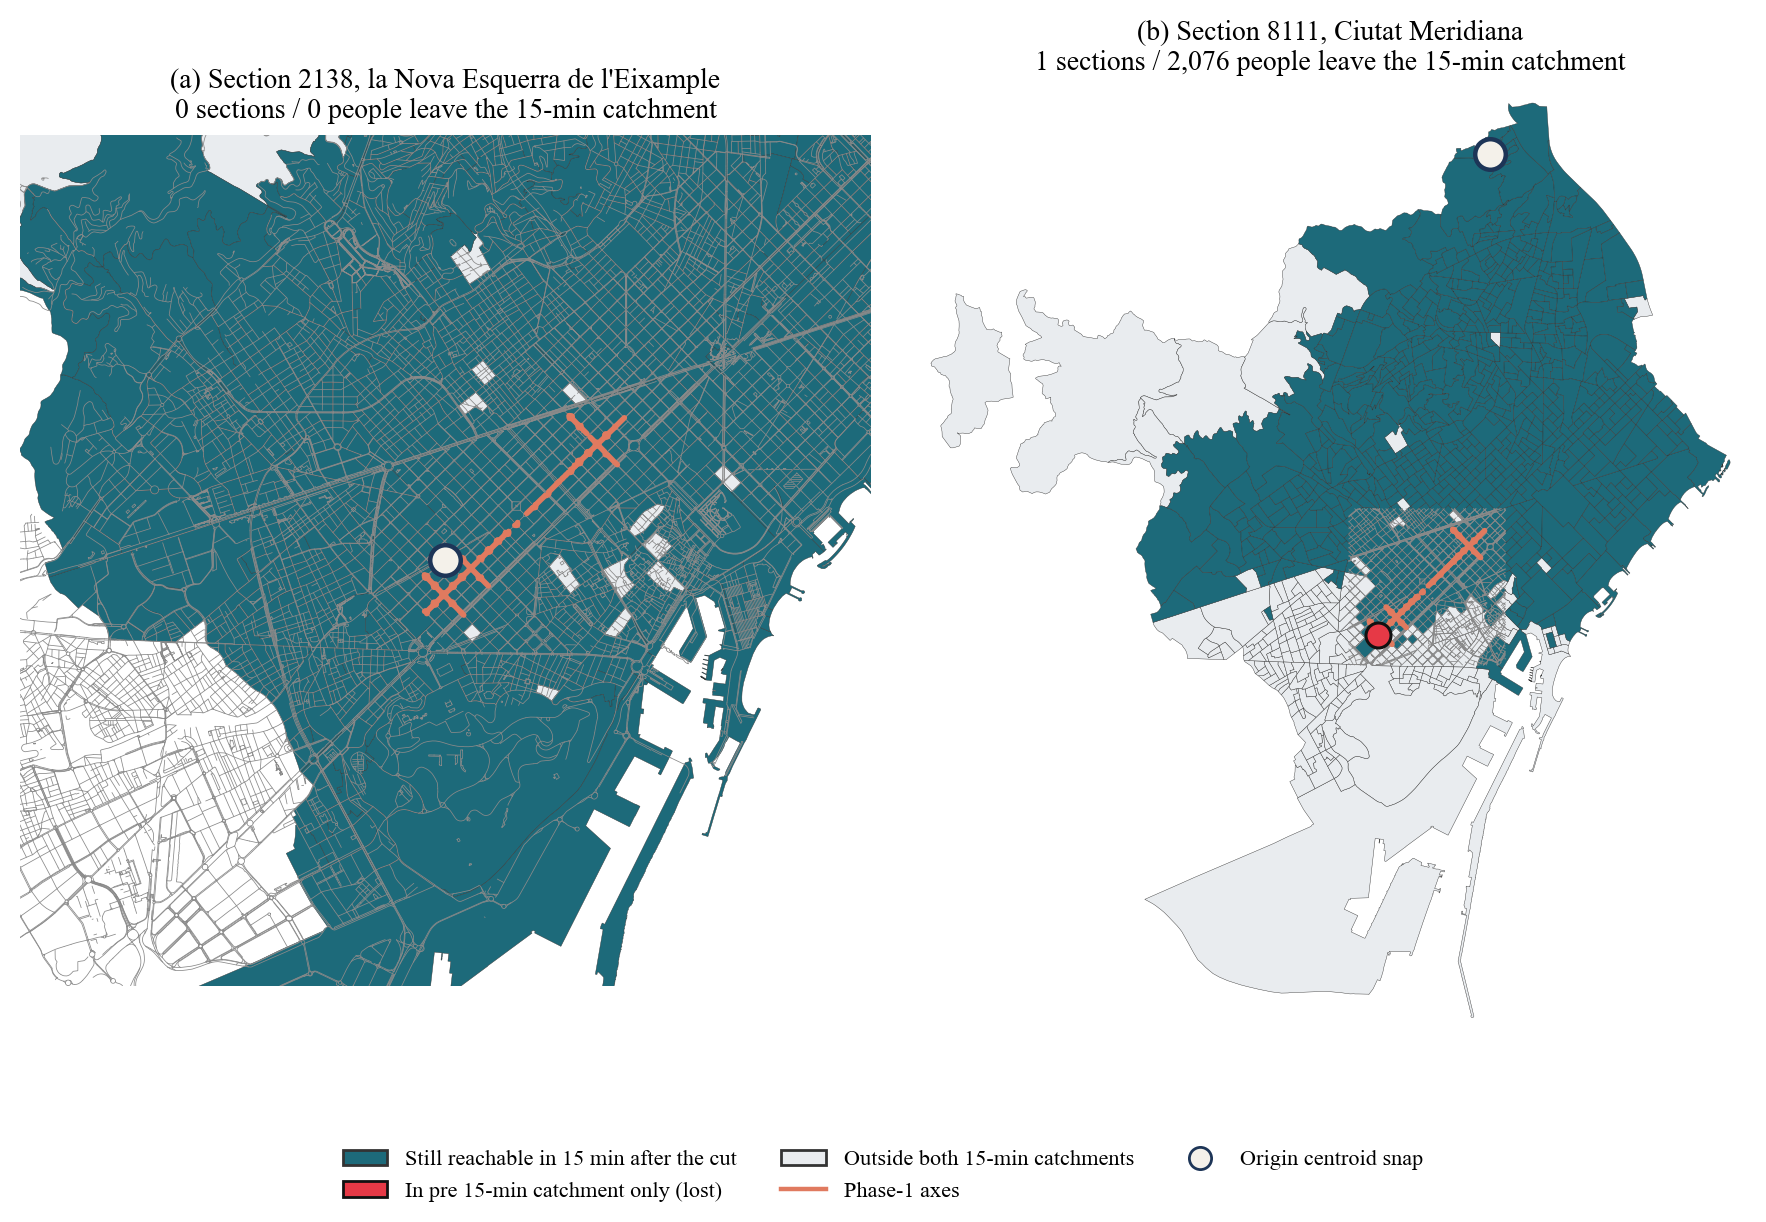
\includegraphics[width=\textwidth,height=0.32\textheight,keepaspectratio]{Fig2_isochrones.png}
\caption{Fifteen-minute car catchments under $\times 100$: still reachable
(teal) and destinations that leave (red). (a)~Section 2138, Nova Esquerra,
loses none. (b)~Section 8111, Ciutat Meridiana, loses one interior section.}
\label{fig:isochrones}
\end{figure*}

\subsection{Off-axis opportunity}

Table~\ref{tab:offaxis} is the city result.

\begin{table}[!htbp]
\centering
\small
\caption{Off-axis median change in estimated car accessibility
($n = 1{,}052$).}
\label{tab:offaxis}
\begin{tabular}{@{}lrr@{}}
\toprule
Measure & Median $\Delta A$ & Median \% \\
\midrule
Car, 15 min, $\times 100$
  & $0$ & $0.00$ \\
Car, 15 min, drop-treated
  & $-1{,}676$ & $-0.10$ \\
Car, 15 min, turns $+15$\,s
  & $0$ & $0.00$ \\
Car, 30 min, $\times 100$
  & $0$ & $0.00$ \\
Hansen $\beta = 0.05$
  & $-220$ & $-0.018$ \\
Walk, 15 min (level)
  & $80{,}632$ & --- \\
\bottomrule
\end{tabular}
\end{table}

No origin gains car access. After local-egress snaps, the 15-minute
$\times 100$ median is $0$ (ten off-axis sections are negative; the rest
sit at the cutoff with no change). Drop-treated is $-0.10\%$ (IQR
$[-0.106,-0.105]$). A stated 15\,s turn penalty on both pre and post graphs
leaves the 15-minute median at $0$ (32 sections negative). Doubling the
turn penalty to 30\,s leaves that median at $0$ (116 sections negative).
Thirty minutes is identically $0$. Hansen at $\beta = 0.05$ is $-0.018\%$
and still shrinks with network distance (correlation $+0.16$).
Stated decays $\beta = 0.03$ and $\beta = 0.15$ give off-axis medians of
$-0.011\%$ and $-0.059\%$ (distance correlations $+0.16$ and $+0.20$);
$\beta = 0.08$ sits between them at $-0.030\%$. Nearby still ranks first.
Moran's $I$ under queen contiguity (999 permutations) is $0.005$
($z=0.53$, $p=0.19$) for $\times 100$, $0.050$ ($z=3.39$, $p=0.016$) for
drop-treated, $0.083$ ($z=6.34$, $p=0.004$) for turns, and $0.162$
($z=9.80$, $p=0.001$) for Hansen. The 15-minute $\times 100$ field is not
distinguishable from spatial randomness: it is essentially unclustered
because it is essentially flat. Table~\ref{tab:bands}
splits the same off-axis rows by network-distance band. Drop-treated is
$-0.10\%$ in every band. $\times 100$ is $0$ in every band.
Fig.~\ref{fig:choropleth} maps 15-minute $\times 100$ (hatched cells are the
15 local-egress snaps, Fig.~\ref{fig:onaxis}) and plots the car post graphs
against network distance. Fig.~\ref{fig:s1} is
the drop-treated choropleth.

\begin{table*}[t]
\centering
\small
\caption{Off-axis median \% change by network distance to a treated node.}
\label{tab:bands}
\begin{tabular}{lrrrrrrr}
\toprule
Band & $n$ & $\times 100$ & IQR & Drop & Hansen & IQR & 30 min \\
\midrule
0--250\,m & 31 & $0.00$ & $[0.00,0.00]$ & $-0.10$ & $-0.033$ & $[-0.32,-0.03]$ & $0.00$ \\
250--500\,m & 42 & $0.00$ & $[0.00,0.00]$ & $-0.10$ & $-0.028$ & $[-0.03,-0.03]$ & $0.00$ \\
500\,m--1\,km & 98 & $0.00$ & $[0.00,0.00]$ & $-0.10$ & $-0.027$ & $[-0.03,-0.02]$ & $0.00$ \\
1--2\,km & 250 & $0.00$ & $[0.00,0.00]$ & $-0.10$ & $-0.023$ & $[-0.03,-0.02]$ & $0.00$ \\
2--3.5\,km & 296 & $0.00$ & $[0.00,0.00]$ & $-0.10$ & $-0.021$ & $[-0.03,-0.02]$ & $0.00$ \\
${>}3.5$\,km & 335 & $0.00$ & $[0.00,0.00]$ & $-0.10$ & $-0.016$ & $[-0.017,-0.016]$ & $0.00$ \\
\bottomrule
\end{tabular}
\end{table*}

\begin{figure*}[t]
\centering
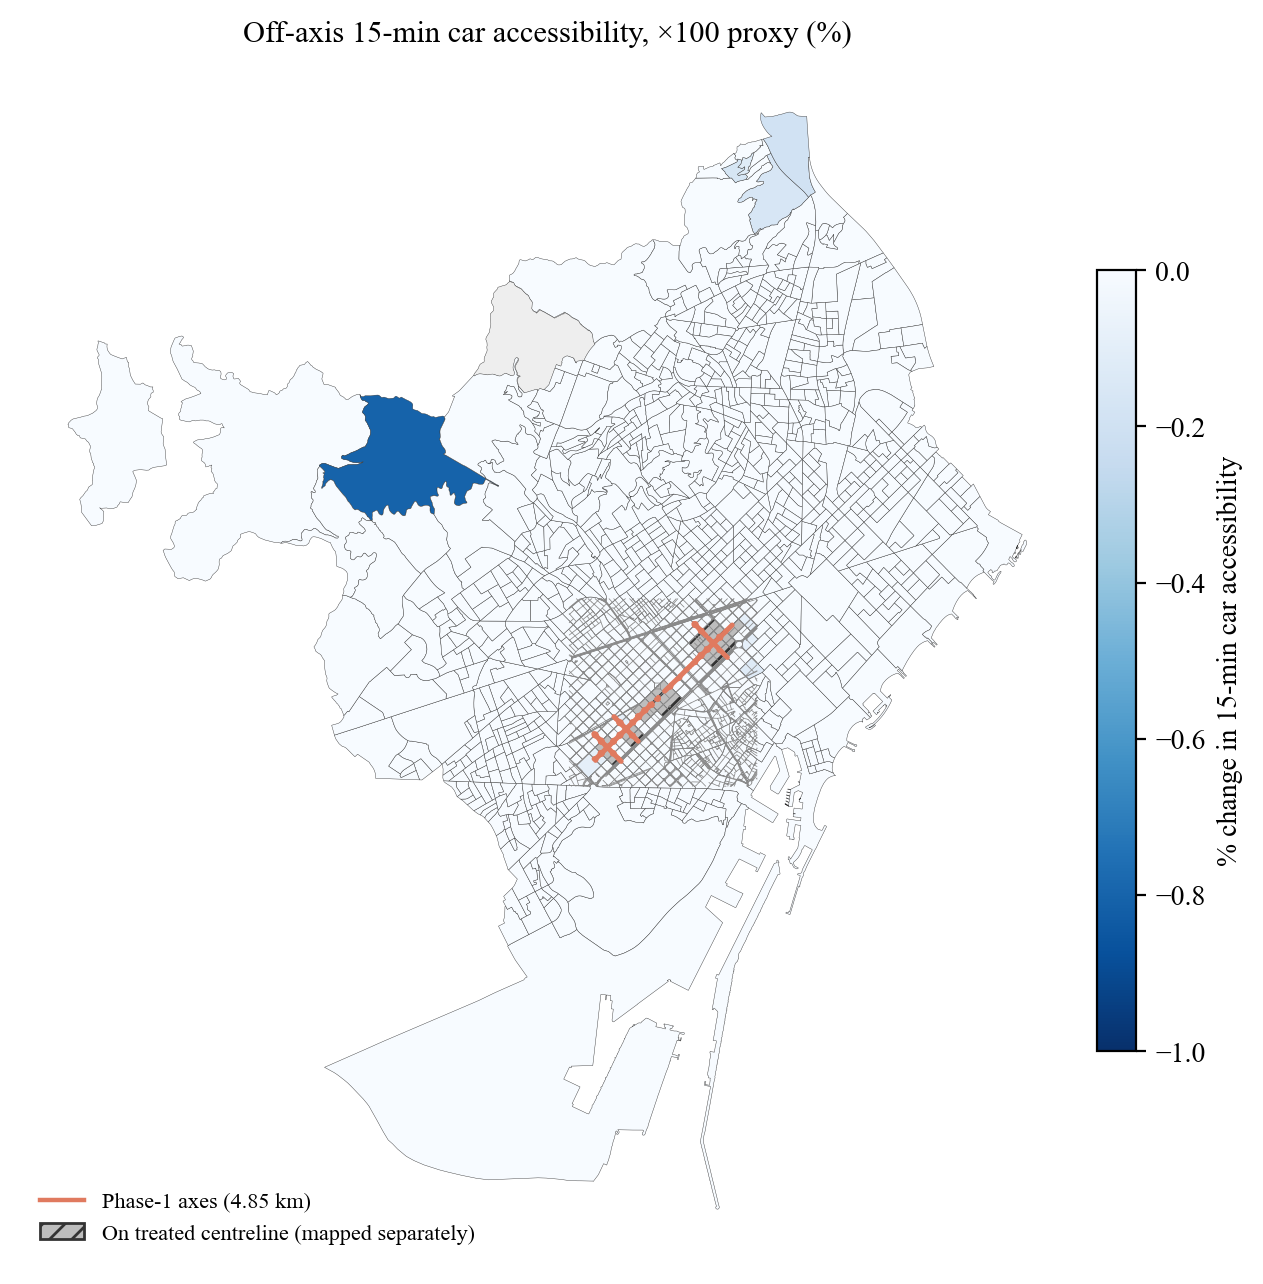
\includegraphics[width=0.48\textwidth]{Fig1_offaxis_car15.png}\hfill
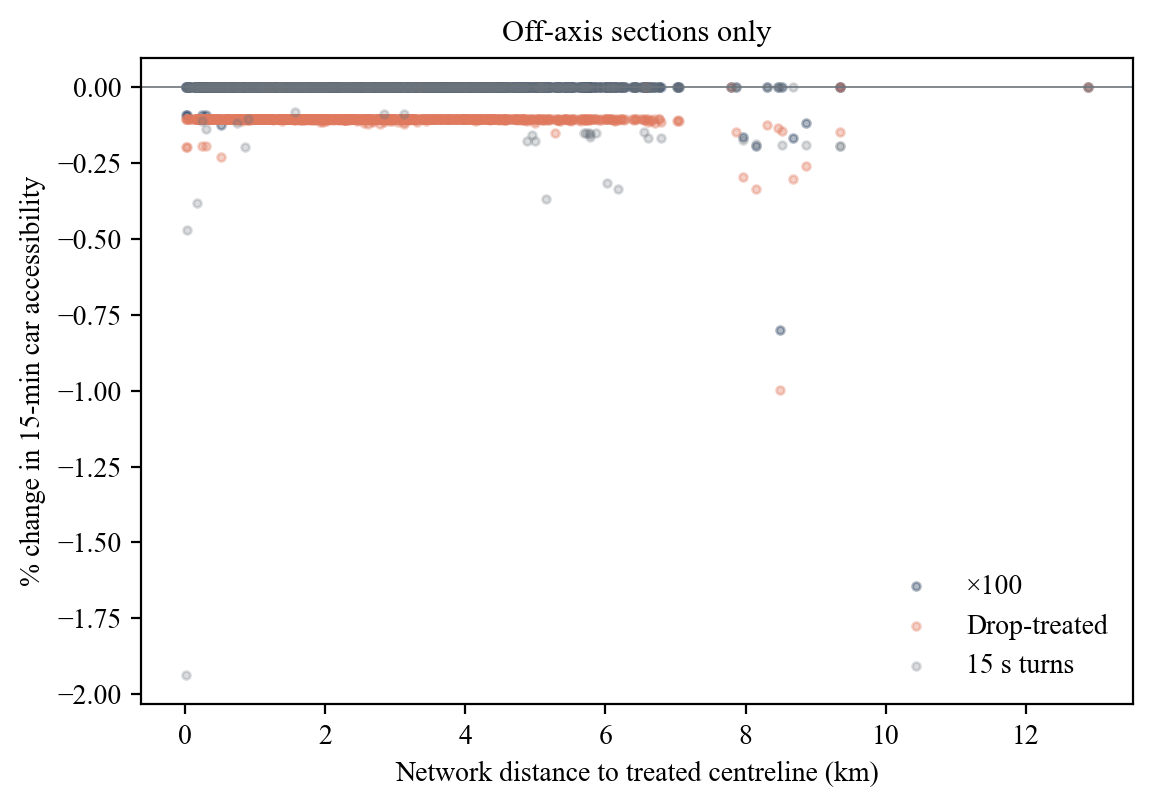
\includegraphics[width=0.48\textwidth]{Fig2_scatter_distance.png}
\caption{Off-axis 15-minute car $\times 100$ (a) and the same \% change
against network distance (b).}
\label{fig:choropleth}
\end{figure*}

\subsection{Incidence by neighbourhood}

Table~\ref{tab:district} reports district medians among off-axis sections.
$\times 100$ is $0$ in every district. Drop-treated is
$-0.10\%$ in every district. Hansen places the larger --- still
sub-$0.12\%$ --- losses on nearby \emph{barris}: Barceloneta ($-0.12\%$),
then Nova Esquerra de l'Eixample ($-0.036\%$), Sants and Les Corts
(Figs.~\ref{fig:hansenmap} and \ref{fig:income}). Fig.~\ref{fig:hansenmap}
uses a tight colour scale (5th percentile $\approx -0.03\%$ to 0) so that a
0.01~percentage-point difference is visible; it is not a second citywide
collapse. Across 73 \emph{barris}, Hansen medians span only $-0.12\%$ to
$-0.012\%$. The $\times 100$ 15-minute ranking of the same neighbourhoods is
essentially flat: Vallbona ($-0.19\%$, $n=1$) and Torre Bar\'o ($-0.08\%$,
$n=2$) are the only \emph{barris} with a non-zero median; the rest sit at
$0$ (Fig.~\ref{fig:s1}b). Correlation of \emph{barri} Hansen \% with
network distance is $+0.29$: farther is smaller loss. That is the incidence
ranking that matches a detour on the grid.

\begin{figure*}[t]
\centering
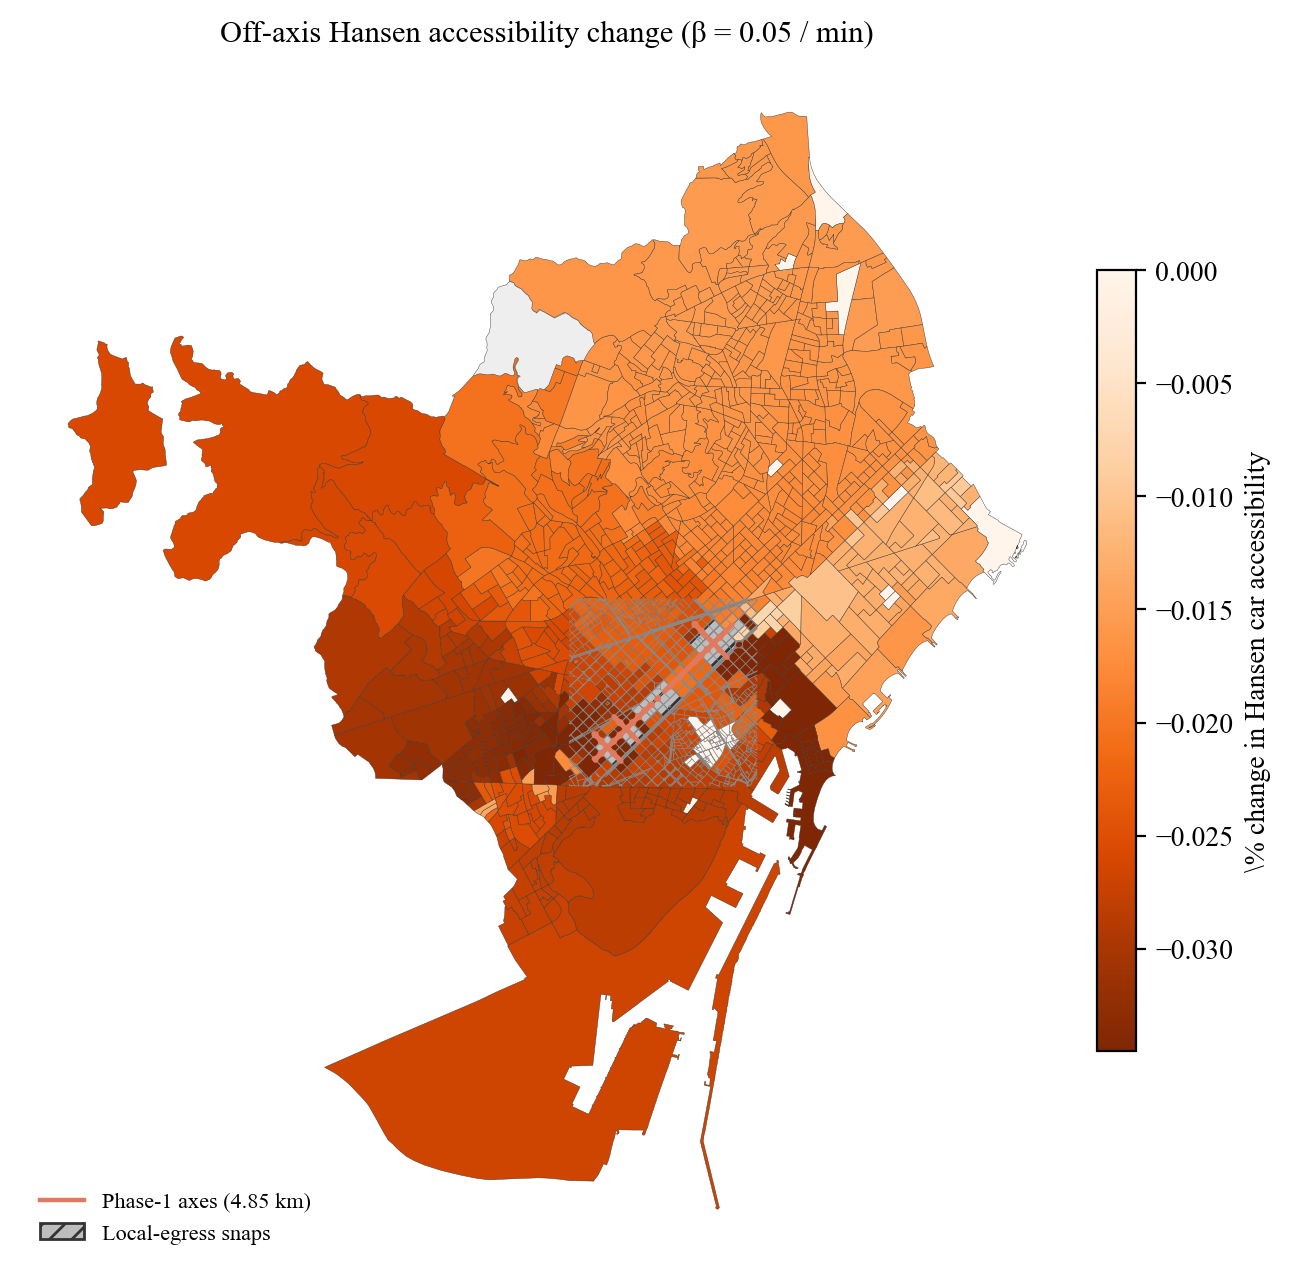
\includegraphics[width=0.58\textwidth]{Fig5_hansen_map.png}
\caption{Off-axis Hansen accessibility change ($\beta = 0.05$ / min).}
\label{fig:hansenmap}
\end{figure*}

Table~\ref{tab:income} splits the same off-axis sections by 2022 household
disposable income per capita. $\times 100$ is $0$ in every quintile.
Drop-treated is $-0.10\%$ in every quintile. Q1 still sits farther
from the axes (median 4.3\,km versus 1.5\,km in Q4); Q5 is slightly farther
than Q4 (2.1\,km) because high-income sections in Sarri\`a--Sant Gervasi sit
off the Eixample grid. Hansen is slightly \emph{larger} in Q5 than in Q1
(Fig.~\ref{fig:income}). The 15-minute map does not inherit a poverty
penalty from this recode.

\begin{table}[!htbp]
\centering
\small
\caption{Off-axis median 15-minute car \% change by district.}
\label{tab:district}
\begin{tabular}{@{}lrrr@{}}
\toprule
District & $\times 100$ & Drop-treated & On-axis \\
\midrule
Sant Andreu              & $0.00$ & $-0.10$ & 0 \\
Nou Barris               & $0.00$ & $-0.10$ & 0 \\
Horta-Guinard\'o         & $0.00$ & $-0.10$ & 0 \\
Sant Mart\'i             & $0.00$ & $-0.10$ & 0 \\
Gr\`acia                 & $0.00$ & $-0.10$ & 0 \\
Sarri\`a--Sant Gervasi   & $0.00$ & $-0.10$ & 0 \\
Ciutat Vella             & $0.00$ & $-0.10$ & 0 \\
Sants-Montju\"ic         & $0.00$ & $-0.10$ & 0 \\
Les Corts                & $0.00$ & $-0.10$ & 0 \\
Eixample                 & $0.00$ & $-0.10$ & 15 \\
\bottomrule
\end{tabular}
\end{table}

\begin{table}[!htbp]
\centering
\small
\setlength{\tabcolsep}{3pt}
\caption{Off-axis income quintiles, 2022 RDLpc.}
\label{tab:income}
\begin{tabular}{@{}lrrrrr@{}}
\toprule
Q & Median EUR & Net km & $\times 100$ & Drop & Hansen \\
\midrule
Q1 lowest  & 16{,}797 & 4.26 & $0.00$ & $-0.10$ & $-0.016$ \\
Q2         & 20{,}438 & 3.08 & $0.00$ & $-0.10$ & $-0.017$ \\
Q3         & 22{,}672 & 2.30 & $0.00$ & $-0.10$ & $-0.018$ \\
Q4         & 25{,}013 & 1.53 & $0.00$ & $-0.10$ & $-0.022$ \\
Q5 highest & 29{,}765 & 2.10 & $0.00$ & $-0.10$ & $-0.025$ \\
\bottomrule
\end{tabular}
\end{table}

\begin{figure*}[t]
\centering
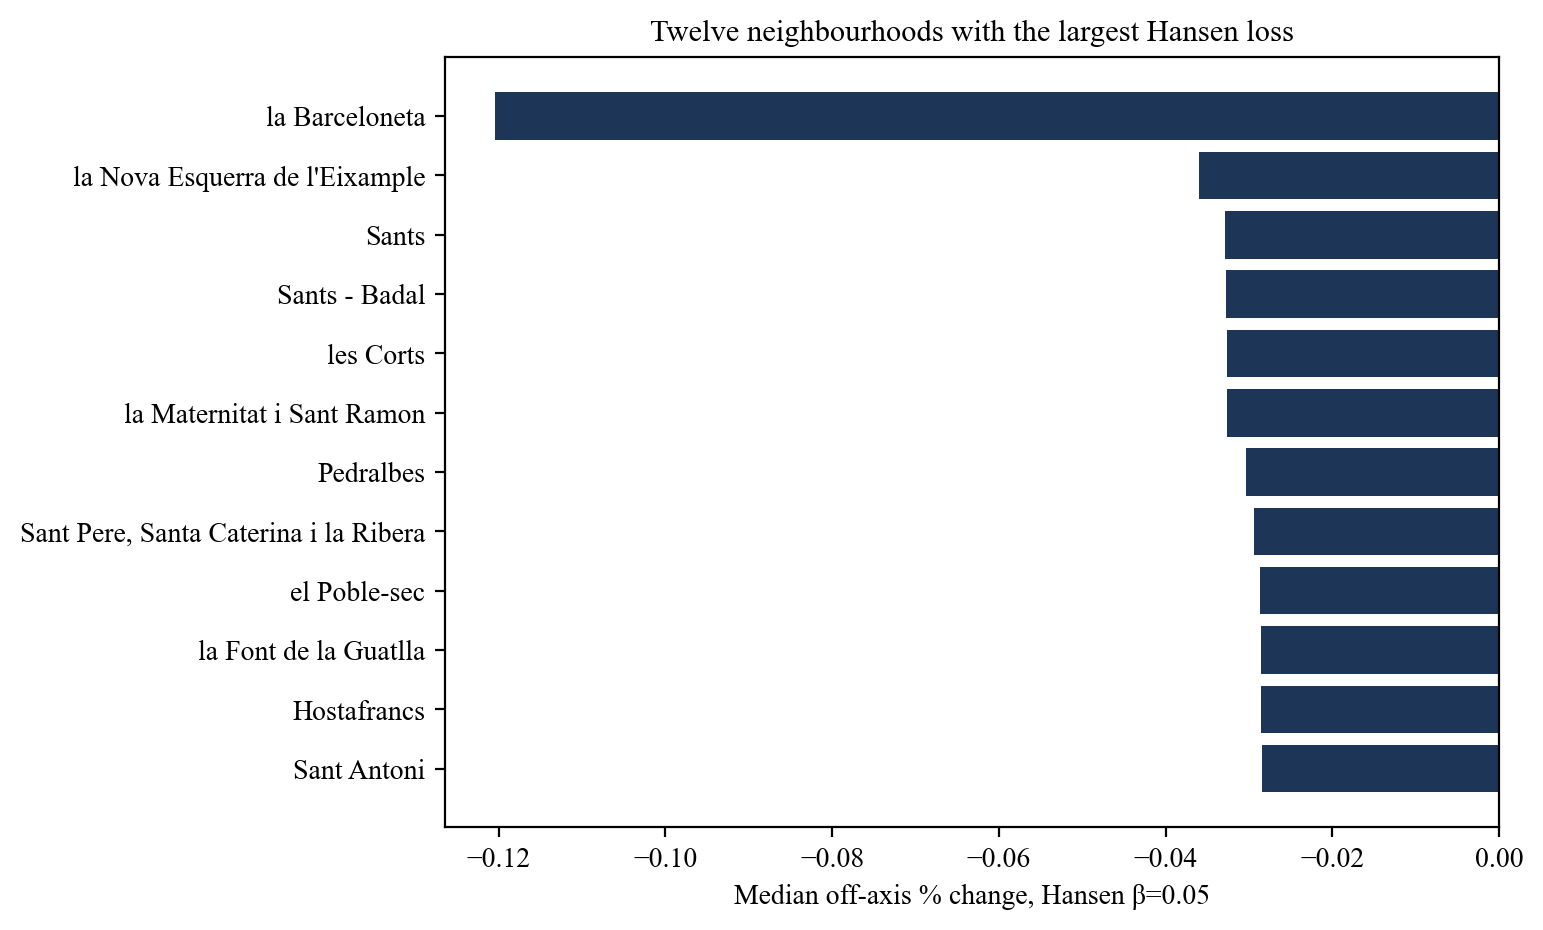
\includegraphics[width=0.48\textwidth]{Fig4_barri_hansen.png}\hfill
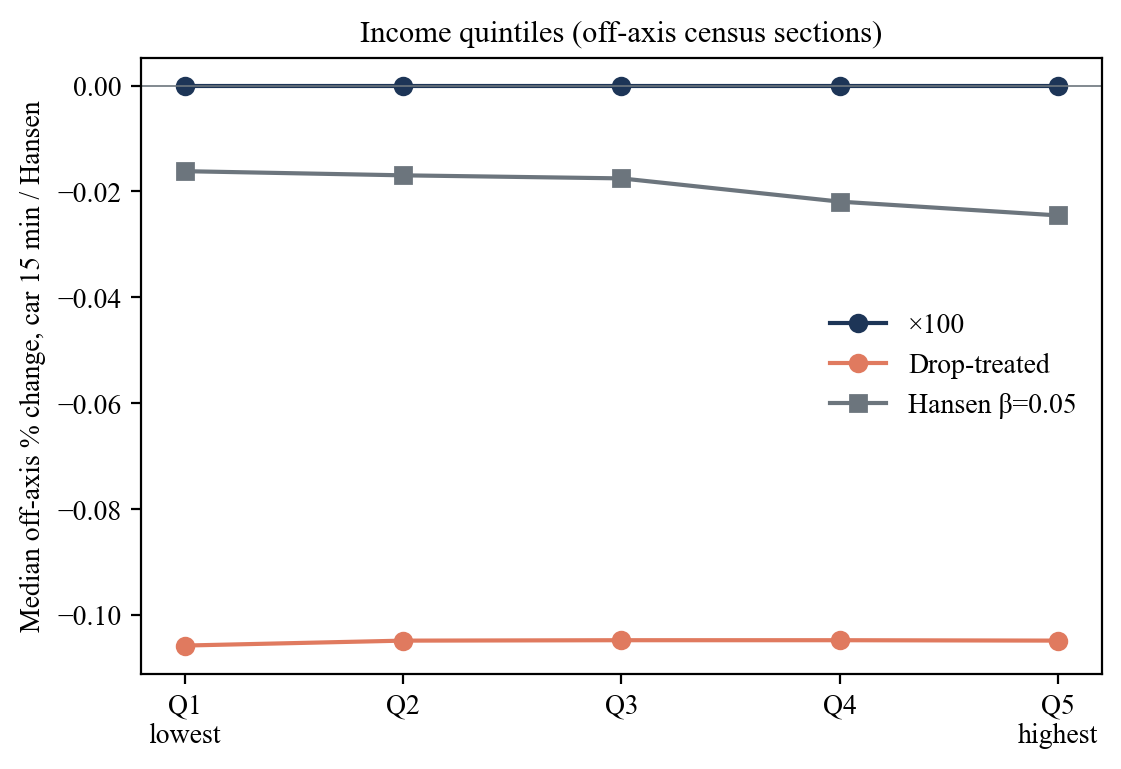
\includegraphics[width=0.48\textwidth]{Fig5_income_quintiles.png}
\caption{Twelve neighbourhoods with the largest median off-axis Hansen loss
(a) and off-axis \% change by income quintile (b).}
\label{fig:income}
\end{figure*}

\subsection{On-axis caveat}

Fifteen sections would have snapped onto the treated centreline, all in
Dreta, Nova Esquerra and Antiga Esquerra de l'Eixample (6, 5 and 4
sections; 23{,}479 residents). Each is connected to the nearest untreated
perpendicular Cerd\`a street within 200\,m (median snap 73\,m) and is excluded from the off-axis
city result. Mixing those 15 rows into the city median would be the same
category error as treating a centroid trapped on the closed street as a
citywide access collapse. They are a local design result: how a resident
leaves a street that no longer through-connects. How a delivery van, an
ambulance, or a resident who cannot walk to that perpendicular uses the
forced-turn squares is not recovered from a census-section centroid, and it
is not estimated here.

Thirteen of the fifteen sit at $0$ under $\times 100$. Two
remain local exceptions (Table~\ref{tab:stubborn}). Section 2093 (Antiga
Esquerra) loses $18\%$ under $\times 100$ and $37\%$ with the 15\,s turn
recode; drop-treated returns it to $-0.22\%$. Section 2070 (Dreta) loses
$7\%$ under $\times 100$ and remains isolated on the drop graph
($-99.9\%$). That is local egress on a street that no longer
through-connects, not a million people becoming unreachable.
Fig.~\ref{fig:onaxis} maps the two scales on separate panels: (a)~the 15
local-egress snaps under $\times 100$ ($-40\%$ to 0); (b)~off-axis sections
within 800\,m ($-2\%$ to 0), with local-egress cells hatched. Section 7097 (Montbau)
is unsnapped on the car graph and is the unshaded hole in
Horta-Guinard\'o; it is not in the off-axis $n = 1{,}052$.

\begin{table}[!htbp]
\centering
\small
\caption{Local-egress sections that remain poorly connected.}
\label{tab:stubborn}
\setlength{\tabcolsep}{3pt}
\begin{tabular}{@{}rlrrrr@{}}
\toprule
Section & \emph{Barri} & Pop. & $\times 100$ & Drop & Turns \\
\midrule
2093 & Antiga Esquerra & 1{,}676 & $-18.1$ & $-0.22$ & $-36.6$ \\
2070 & Dreta & 1{,}270 & $-7.1$ & $-99.9$ & $-24.0$ \\
\bottomrule
\end{tabular}
\end{table}

\begin{figure*}[t]
\centering
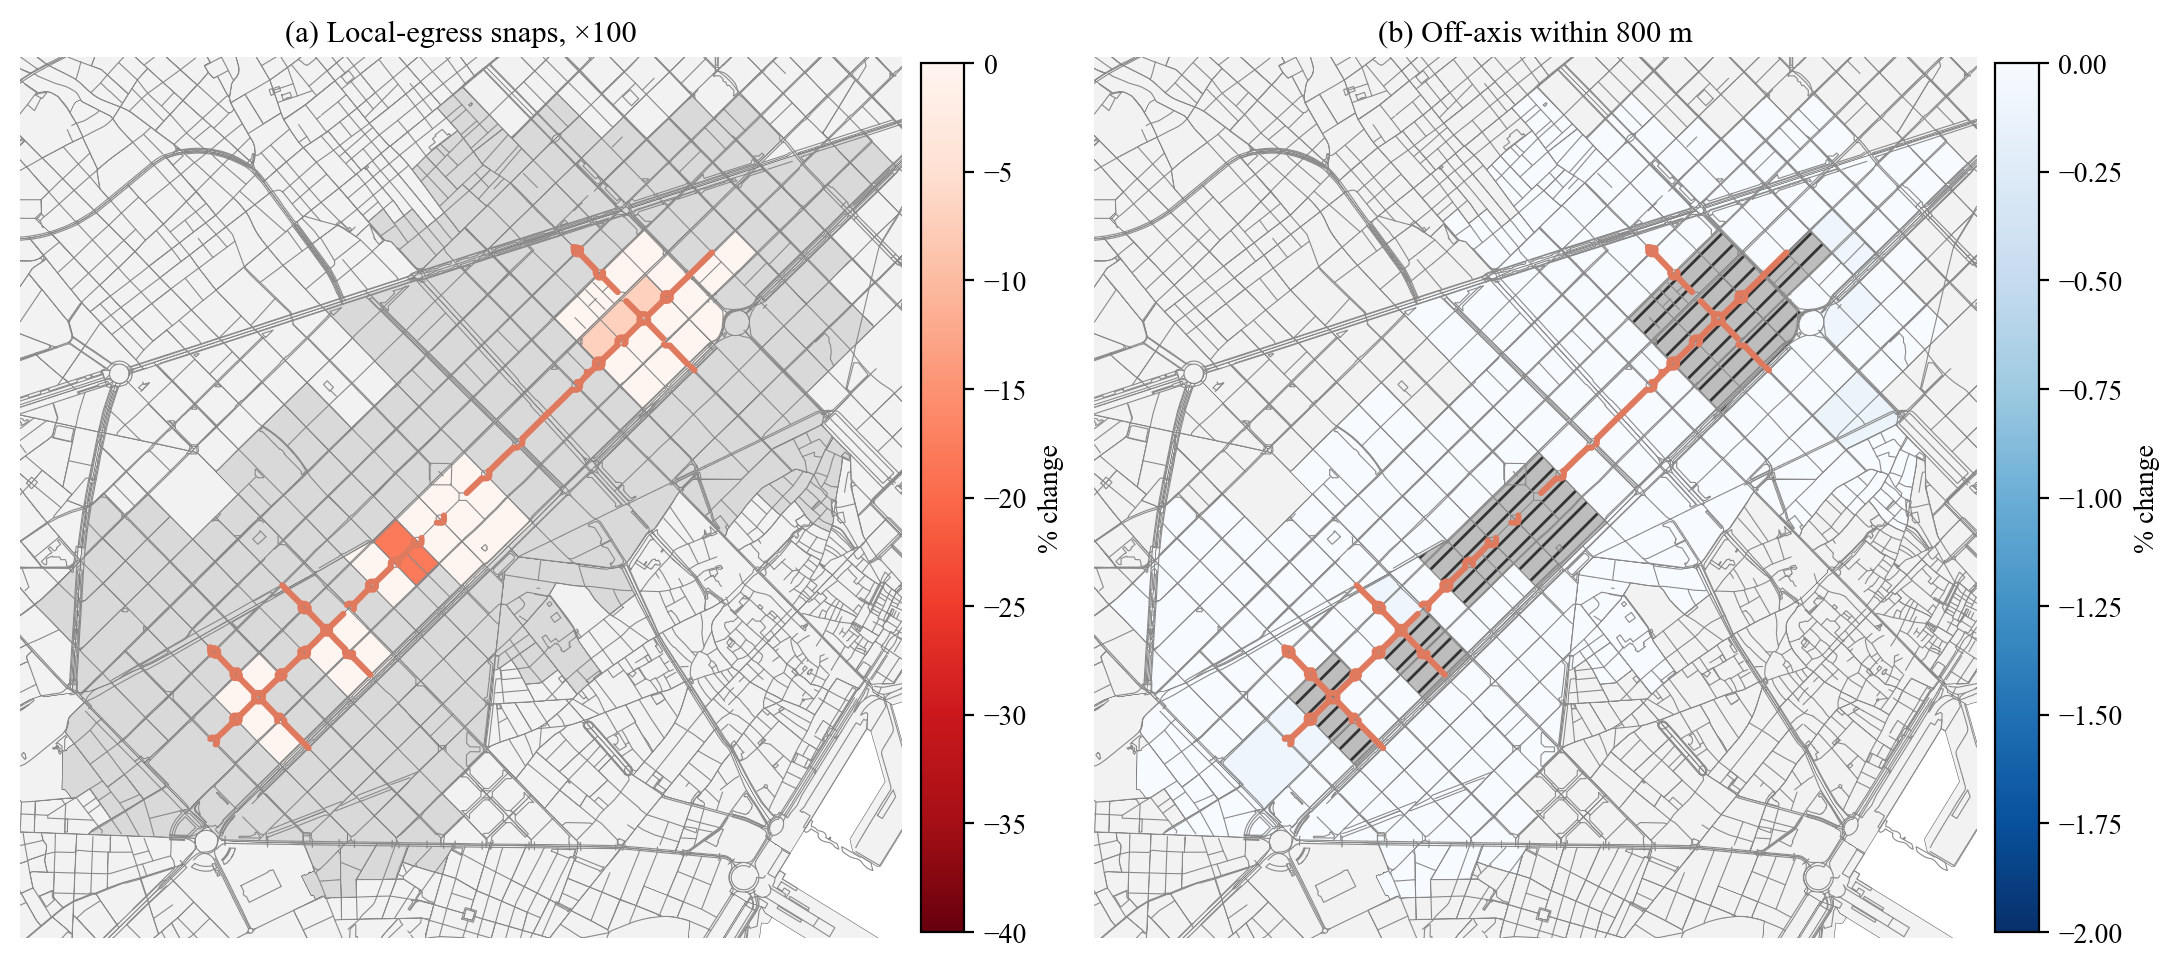
\includegraphics[width=\textwidth,height=0.28\textheight,keepaspectratio]{Fig3_onaxis_x100.png}
\caption{Local-egress snaps under $\times 100$ (a) and nearby off-axis (b).}
\label{fig:onaxis}
\end{figure*}

\subsection{Walk}

Median 15-minute walk opportunity is 80{,}632 residents (median 24
destination sections). The walk graph is not recoded, so walk $A_i$ is a
level, not a pre/post change. Benches, trees, square geometry, pedestrian
level of service and crossing time are not in the impedance. A stated
pedestrian scenario would recode the injected centreline as a walkable link
and would have to be labelled simulated. That scenario is not in this
article, and qualitative active-mobility gains are not inferred from an
unchanged walk graph.

%==============================================================================
\section{Discussion}
\label{sec:disc}

On the Cerd\`a grid, recoding 4.85\,km of through-movement does not close
car access to other residents. Off-axis 15-minute opportunity is $0$ under a
punitive $\times 100$ prohibition, $-0.10\%$ when the axis is taken out of
the car graph, and $0$ when a stated 15\,s penalty sits on every
non-through turn, pre and post. The corridor itself adds 0.7 minutes on
link time and 1.1 minutes with turns. A 30\,s turn penalty still leaves
the off-axis 15-minute median at $0$. Those are small numbers, and they are
the result for this grid. They are not a result about low-traffic
neighbourhoods on dendritic streets
\citep{Thomas2024,Verlinghieri2025} or about a temporary pedestrianisation
on a less redundant network \citep{Parady2025}.

The geographical work is to stop the 15-minute map from being read as a
periphery penalty, and to stop a near-ceiling 15-minute field from being
read as proof that the cut did nothing. Cumulative opportunity at a round
threshold will always first drop the people who were already far --- if
destinations remain trapped on the treated centreline. Once those 15
centroids leave by an untreated perpendicular, Fig.~\ref{fig:isochrones}b no
longer darkens: one interior section, 2{,}076 people, leaves the Ciutat
Meridiana catchment. That cell sits in the centre of Barcelona, not at the
municipal edge and not in an omitted first-crown municipality. A first-crown
$O_j$ would raise the level of $A_i$ at the rim, including from Sants and
Nou Barris; it would not move the destination that leaves. Hansen and the
drop-treated graph all say the detour, such as it is, sits near the cut. A
singular reliance on the uncorrected cumulative indicator would capture zero
spatial variance, because the 15-minute $\times 100$ field is flat
\citep{Moreno2021,Pozoukidou2021,Handy2020}. That flatness is the ceiling of
a 15-minute free-flow catchment on this municipal graph, plus a small
detour; Hansen is the ranking that is not at that ceiling. Drop-treated sits $0.10$
percentage points below $\times 100$ because deleting the treated edges
isolates one local-egress node (section 2070); $\times 100$ keeps that
node in the graph at a punitive cost, so the off-axis median does not
inherit that local isolation.

The income table is the same warning in another register. $\times 100$ is
$0$ in every quintile. Drop-treated is $-0.10\%$ in every quintile. Hansen
is slightly larger in Q5. Equity as
incidence \citep{Pereira2017,Lucas2012,Martens2017} does not license reading
a cutoff ranking as a poverty penalty. If a workplace layer concentrated
employment next to the axes, that ranking could change; it has not been
shown here.

Three limits are binding. Opportunities are municipal residents, not jobs,
amenities, or the adjacent first crown; a workplace or metropolitan layer
would change \emph{levels} of $A_i$ and might change incidence. Peripheral
sections (Sants, Nou Barris) can reach L'Hospitalet, Santa Coloma or Sant
Adri\`a in 15 minutes of free-flow time; those residents are not in $O_j$,
so the \emph{level} of $A_i$ at the rim is truncated by design. The
destination that leaves the Ciutat Meridiana catchment is inside Barcelona,
so that truncation does not manufacture the cutoff artefact. Times are
free-flow link cruise times on one contemporary OSM extract, plus a stated
15\,s non-through turn, without congested assignment. Hansen $\beta$ is a
ranking check, not a trip-length fit. If junction delay on the remaining
grid were large, or if a user-equilibrium assignment put delay beyond the
stated recodes, car $\Delta A$ would be more negative than reported here.
Walk and cycle gains remain unmeasured until a stated recode or a GTFS
layer exists. None of those limits licenses quoting the city-mean
$\Delta A$, which is a local-egress $\times 100$ artefact, or colouring the
municipality with origins that sit on the closed centreline.

For practice the implication is narrow and usable. A dense orthogonal grid
can absorb a permanent mid-block through-cut with a small simulated loss of
residential interaction potential for almost every off-axis census section.
That is not an argument that volumes did not fall, and it is not an
argument that walking improved. It is an argument that access and volume
are different objects. Cities that want to know whether they sacrificed
access --- and to answer the consultation claim that residents will be
trapped behind a new green axis --- should publish off-axis median
$\Delta A$ under more than one impedance, with centroids leaving by an
untreated perpendicular rather than sitting on the closed centreline. The
15-minute map is admissible if, and only if, a Hansen or drop-treated map
is printed next to it. The local-egress snap is a local design question
--- how a resident leaves a street that no longer through-connects ---
and belongs in the consultation pack as such.

\section{Conclusion}
\label{sec:conc}

Barcelona's first permanent green axes remove through traffic on 4.85\,km of
the Eixample grid. On a counterfactual recode of a single contemporary
OpenStreetMap extract, simulated car travel time along that corridor rises by
0.7 minutes on link time and 1.1 minutes with a stated 15\,s turn penalty.
Estimated 15-minute car accessibility among off-axis sections is $0$ under
a $\times 100$ treated-edge prohibition, $-0.10\%$ when those edges are
dropped, and $0$ when the same 15\,s turn sits on both pre and post graphs
(still $0$ at 30\,s).
A Ciutat Meridiana origin loses one destination section, in the centre, at
the rim of a 15-minute trip. Hansen's ranking is nearby, not peripheral.
Once local-egress snaps replace centroids trapped on the treated
centreline, the 15-minute map is flat. Access to other residents, on this
evidence and on this grid, is not the same object as traffic volume, and it
is not sacrificed at city scale by this recode. Off-axis median $\Delta A$
under more than one impedance, with local egress, is what a consultation
document needs if the political question is whether residents are trapped.

%==============================================================================
\section*{CRediT authorship contribution statement}
%==============================================================================

\noindent\textbf{Seshadri Naik Moode:} Conceptualization; Methodology;
Software; Formal analysis; Validation; Visualization; Writing -- original
draft; Writing -- review \& editing.

\section*{Declaration of competing interest}

The author declares that he has no known competing financial interests or
personal relationships that could have appeared to influence the work reported
in this paper.

\section*{Funding}

This research has been partially funded by the Spanish Ministry of Economy
and Competitiveness (Ministerio de Econom\'{i}a y Competitividad, Gobierno
de Espa\~{n}a), Grant ref.\ PID2019-105331RB-I00, number J-02653 Platoon.
Publications and other results are supported by the JOAN OR\'{O} FI
AGAUR-2022 grant num.\ FI\_B 00597 of the Secretariat for Universities and
Research of the Department of Research and Universities of the Generalitat
de Catalunya and the European Social Fund Plus.

\section*{Ethics statement}

This study uses publicly released census-section population, neighbourhood
boundaries and OpenStreetMap. No human-subject data were collected.
Institutional ethics approval was not required.

\section*{Data availability}

Census-section geometries and 2022 \emph{padr\'o} population are from Open
Data BCN. The street network is OpenStreetMap (extract 7 September 2026).
As-built phase-1 centrelines, graphs, accessibility scores, robustness
tables and the Python scripts that reproduce numbered tables and figures are
available from the corresponding author and will be deposited in an open
repository upon acceptance. Traffic counts were not used.

\section*{Declaration of generative AI in scientific writing}

During the preparation of this work the author used language-model assistance
(Cursor) in order to draft and edit the manuscript. After using this tool, the
author reviewed and edited the content as needed and takes full responsibility
for the content of the publication.

\appendix
\setcounter{figure}{0}
\renewcommand{\thefigure}{A.\arabic{figure}}
\section{Additional maps}
\label{app:s1}

Drop-treated 15-minute change and the $\times 100$ neighbourhood ranking
are mapped here so they are not mixed into the city result in
Section~\ref{sec:results}.

\begin{figure*}[t]
\centering
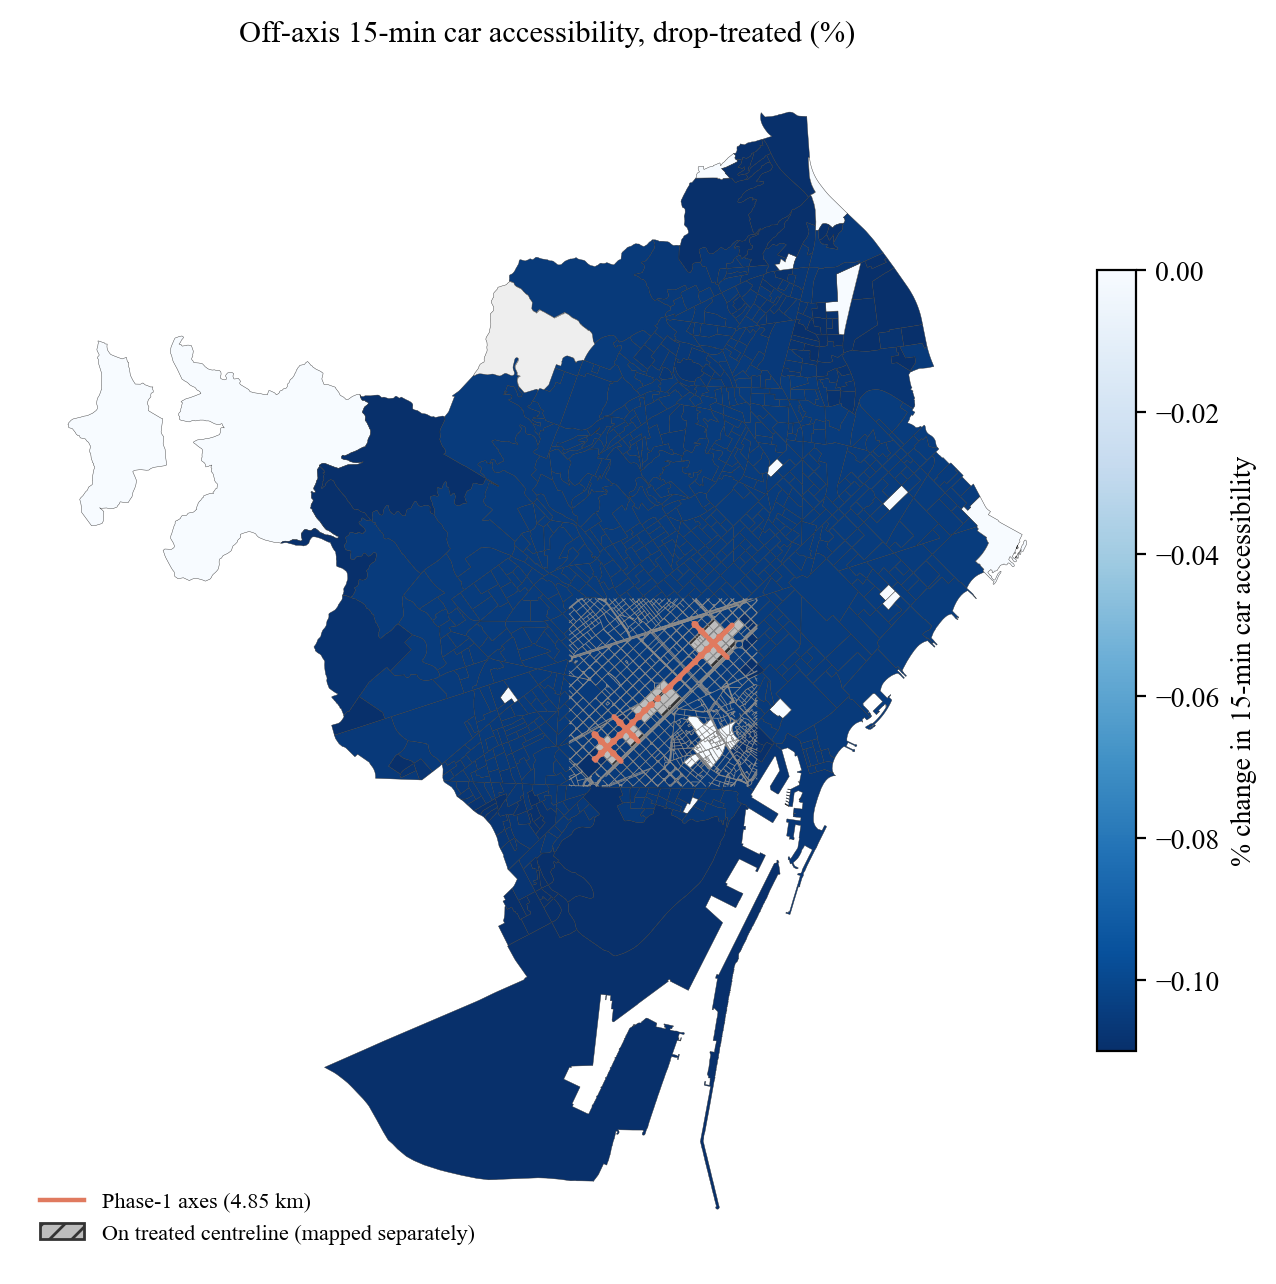
\includegraphics[width=0.48\textwidth]{FigS1_offaxis_drop.png}\hfill
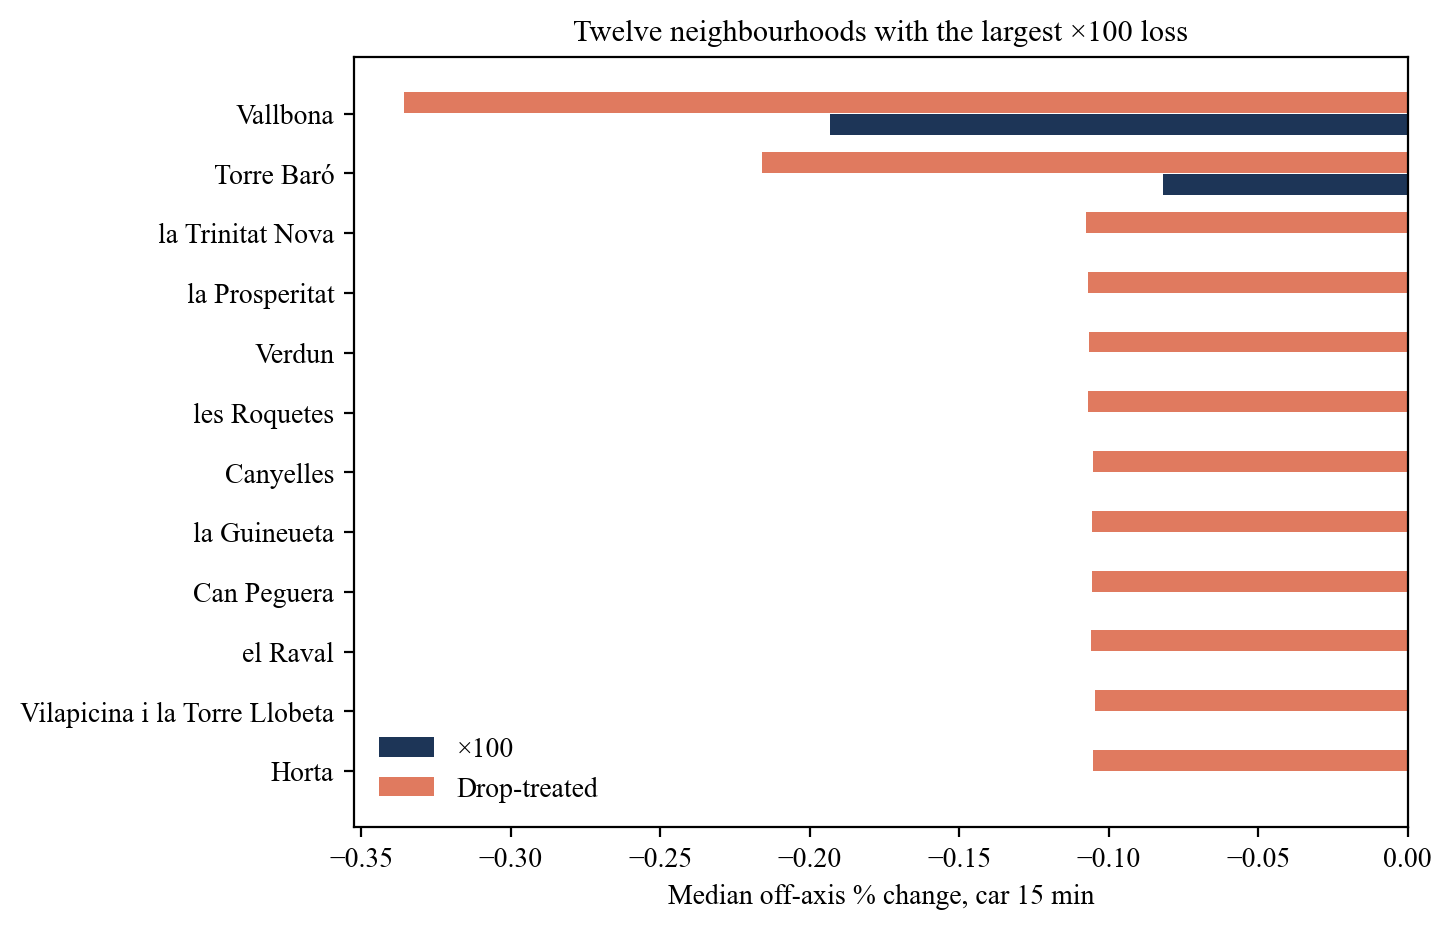
\includegraphics[width=0.48\textwidth]{FigS2_barri_x100.png}
\caption{Drop-treated 15-minute car \% change, off-axis (a), and the twelve
neighbourhoods with the largest median off-axis $\times 100$ loss (b).}
\label{fig:s1}
\end{figure*}

\bibliographystyle{cas-model2-names}
\bibliography{references}

\end{document}
